\documentclass{beamer}
\usepackage[utf8]{inputenc}
\usepackage[T1]{fontenc}
\usepackage[french]{babel}
\usepackage{hyperref}
\usepackage{graphicx}
\usepackage{amsmath,amssymb}
\usepackage{tabularx}
\usepackage{booktabs}
\usepackage{minted}
%\usepackage[compatibility=false]{caption}
%\usepackage{subcaption}

\newcolumntype{Y}{>{\centering\arraybackslash}X}

\usetheme[numbering=fraction,block=fill,progressbar=frametitle]{metropolis} %Use metropolis theme

%\setbeamertemplate{blocks}[rounded]
\title{Deep learning : votre propre cerveau artificiel avec Python}
\date[15 octobre 2016]{15 octobre 2016}
\author[\url{https://nicolas.audebert.at}]{Nicolas Audebert (\href{https://twitter.com/nshaud}{@nshaud})}
\institute{\href{mailto:nicolas+python@audebert.at}{nicolas+python@audebert.at}}
\titlegraphic{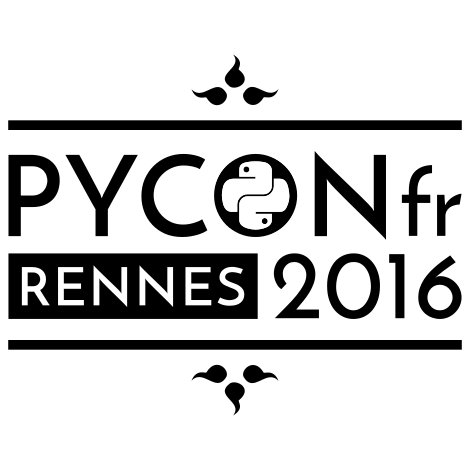
\includegraphics[width=0.3\textwidth]{pycon}}
\begin{document}


\setmainfont{Fira Sans}
\maketitle

\begin{frame}
\tableofcontents
\end{frame}

\section{C'est quoi le deep learning ?}

\begin{frame}{Du cortex visuel\dots}  
Le cortex visuel des mammifères est constitué de neurones qui :
\begin{itemize}
	\item calculent des convolutions (\textit{aka} des filtres),
    \item génèrent des représentations abstraites,
    \item \textit{via} des activations neuronales (impulsions électriques).
\end{itemize}
\begin{figure}
 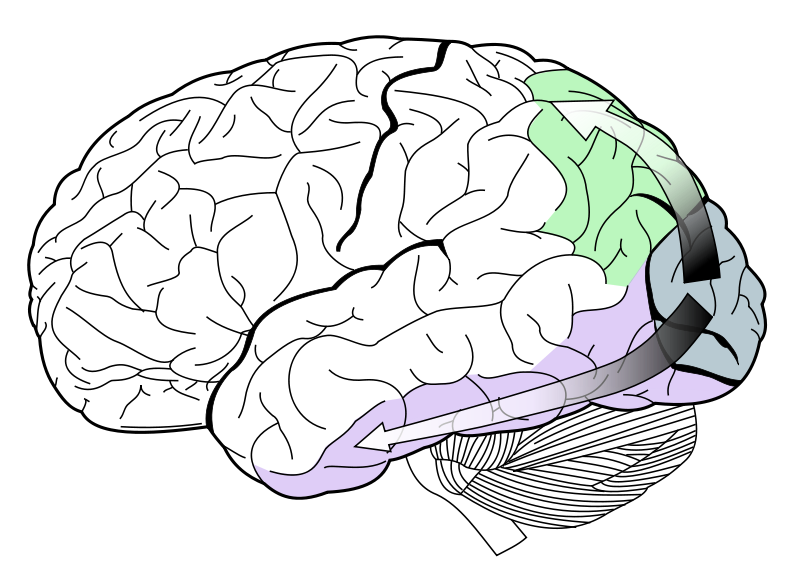
\includegraphics[width=0.4\textwidth]{cortex}\\
 \tiny{Par Selket, CC BY-SA 3.0, \url{https://commons.wikimedia.org/w/index.php?curid=1679336}}
\end{figure}
\end{frame}

\begin{frame}{Du cortex visuel\dots}
\begin{figure}
	
\includegraphics[width=\textwidth]{visual_cortex_task}
\end{figure}
\begin{block}{Comment ?}
Le cerveau sait transformer l'image pour répondre à :
\begin{itemize}
	\item "Où ?" : localisation
    \item "Quoi ?" : sémantique
\end{itemize}
\end{block}
\end{frame}

\begin{frame}{Du cortex visuel\dots}
\begin{figure}
	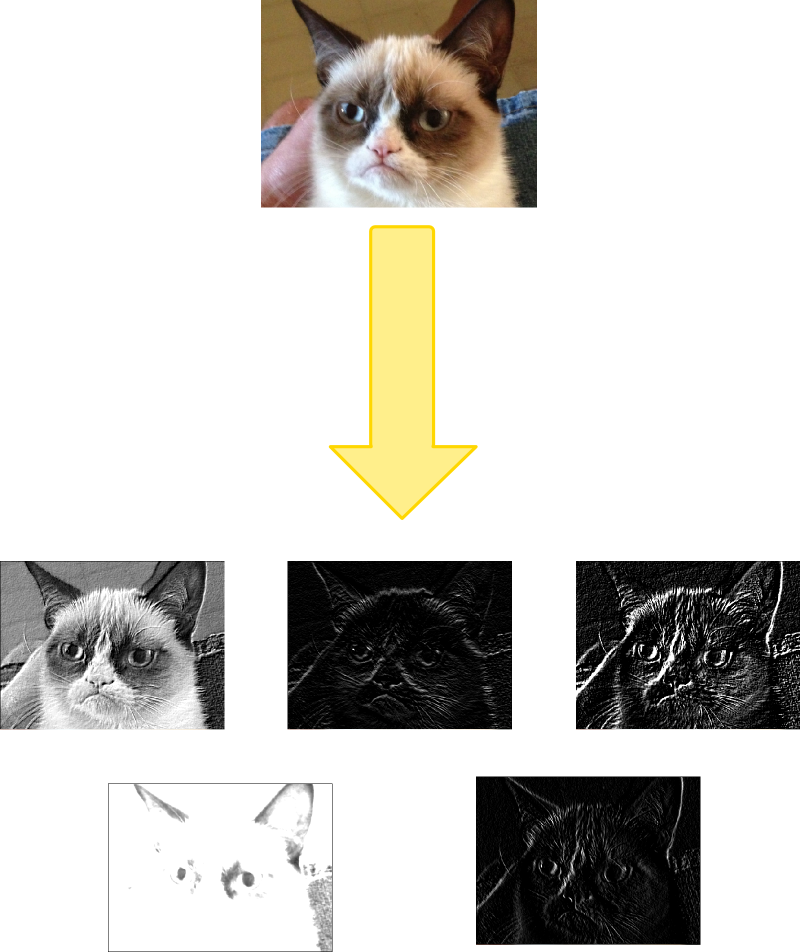
\includegraphics[width=0.5\textwidth]{filters}
\end{figure}
\end{frame}

\begin{frame}{Vers un modèle mathématique}  

L'activation d'un neurone peut se traduire par la transformation (non-linéaire) d'une entrée en une sortie (une \textit{fonction de transfert}).

\begin{figure}
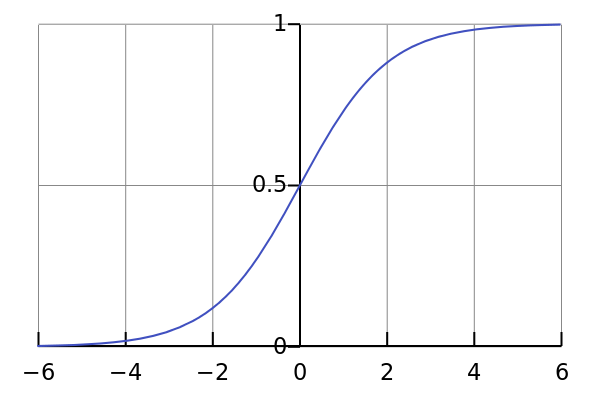
\includegraphics[width=0.6\textwidth]{sigmoid}\\
\tiny{\url{https://commons.wikimedia.org/wiki/File:Logistic-curve.svg}}
\end{figure}
\end{frame}

\begin{frame}{Vers un modèle mathématique}
Exemple de convolution :
\begin{figure}
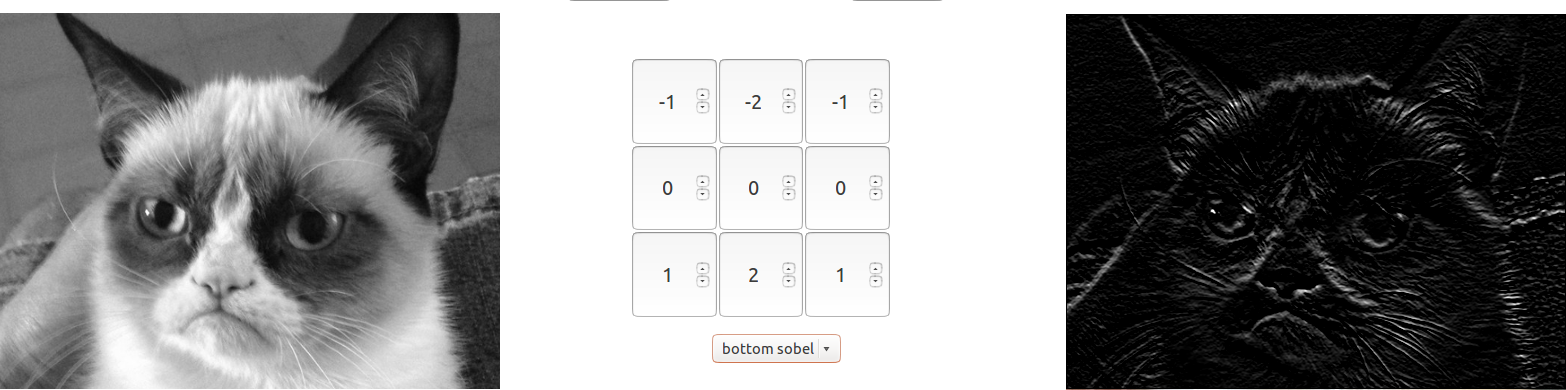
\includegraphics[width=\textwidth]{bottom_sobel}\\
\tiny{\url{http://setosa.io/ev/image-kernels/}}
\end{figure}
\end{frame}

\begin{frame}{Vers un modèle mathématique}  

Simuler des neurones artificiels ? C'est possible !

\end{frame}

\begin{frame}{L'apprentissage automatique}
\begin{block}{À quoi ça sert ?}
Rendre l'ordinateur capable\dots  d'apprendre !
\end{block}

\begin{block}{Comment ?}
Grâce à l'apprentissage par l'exemple
\end{block}
\end{frame}

\begin{frame}{Pour quelles tâches ?}
\begin{block}{Bas niveau}
\begin{itemize}
	\item Reconnaissance vocale
    \item Détection d'objets
    \item Études statistiques
\end{itemize}
\end{block}

\begin{block}{Haut niveau}
\begin{itemize}
	\item Conduite autonome
    \item Jeu de Go
    \item Traduction en temps réel
\end{itemize}
\end{block}

\end{frame}

\begin{frame}{Principe de l'apprentissage}
Minimiser l'erreur entre une prédiction et la vérité
\end{frame}

\begin{frame}{Exemples}
AlphaGo, Autopilot Tesla, Google Translate, Prisma, \dots
\end{frame}

\section{Outils, techniques et applications}

\begin{frame}{Idée générale}  
\begin{itemize}
	\item On définit une \textbf{architecture} (ou topologie) de réseau de neurones artificiels.
    \item On \textbf{apprend} (optimise) les poids des connexions entre neurones.
    \item Pour \textbf{minimiser} l'erreur entre prédiction et objectif.
\end{itemize}

\begin{alertblock}{Différentes architectures pour différentes tâches}
L'architecture choisie dépend du format d'entrée (texte, image\dots) et de la tâche à réaliser (détection, classification\dots).
\end{alertblock}
\end{frame}

\begin{frame}{Réseau de neurones "entièrement connecté"}  
\begin{figure}
	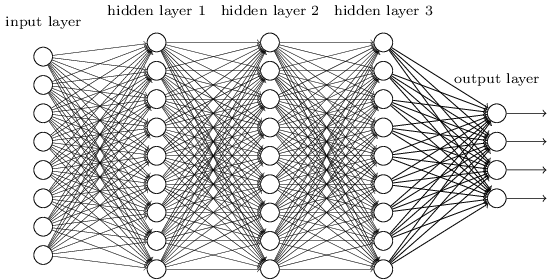
\includegraphics[width=0.8\textwidth]{fully_connected}\\
    \tiny{Michael A. Nielsen, "Neural Networks and Deep Learning", CC-NC-3.0}
\end{figure}
\centering
\begin{itemize}
	\item \textbf{entrée} = vecteur 1D, \textbf{sortie} = vecteur 1D
    \item exemple : classer homme/femme en fonction d'un vecteur de préférences de films
 \end{itemize}
\end{frame}

\begin{frame}{Réseau de neurones "convolutif"}  
\begin{figure}
	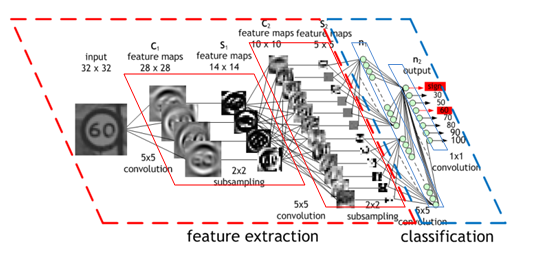
\includegraphics[width=\textwidth]{convnet}\\
    \tiny{Maurice Peemen, \url{https://devblogs.nvidia.com/parallelforall/deep-learning-nutshell-core-concepts/}}
\end{figure}
\begin{itemize}
	\item \textbf{entrée} = image (matrice 2D), \textbf{sortie} = vecteur 1D
 \end{itemize}
\end{frame}

\begin{frame}{Auto-encodeurs}
\begin{figure}
	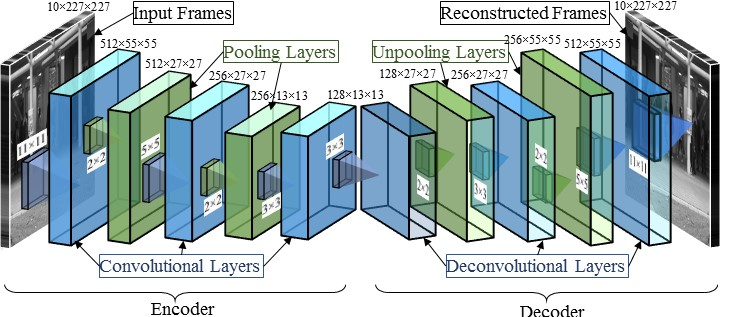
\includegraphics[width=\textwidth]{autoencoder}\\
    \tiny{Hasan et al., "Learning Temporal Regularity in Video Sequences"}
\end{figure}
\begin{itemize}
	\item \textbf{entrée} = n'importe, \textbf{sortie} = même que l'entrée
    \item représentation au \textbf{milieu} = \textbf{compression}, débruitage\dots
\end{itemize}
\end{frame}

\begin{frame}{L'analyse d'image}
\begin{figure}
	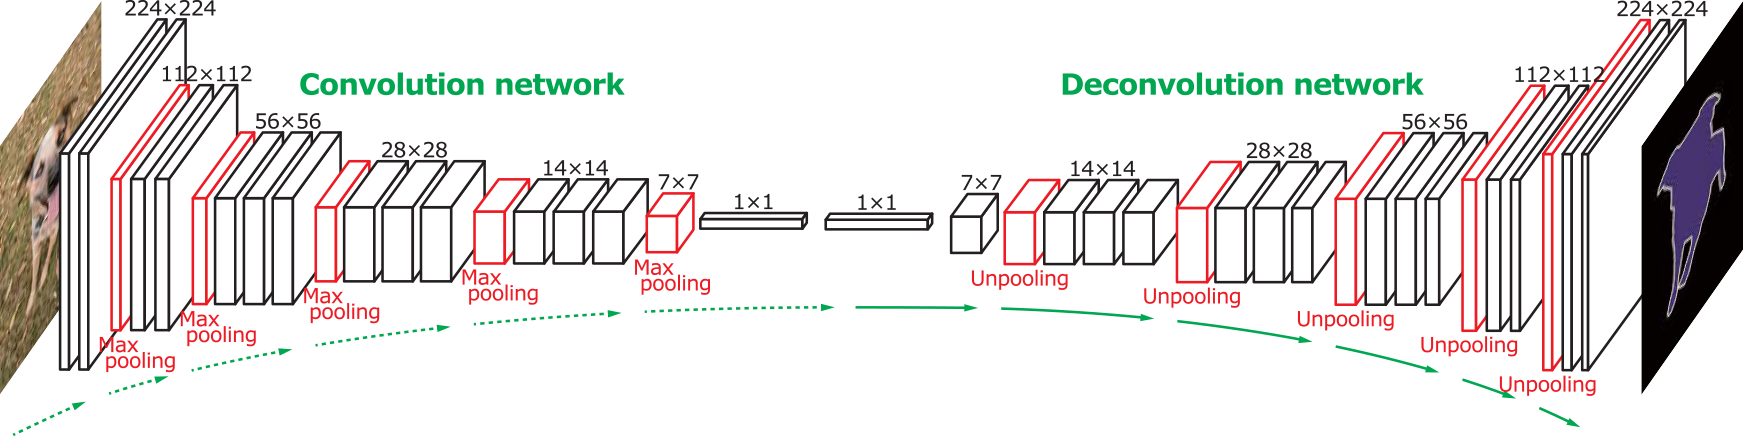
\includegraphics[width=\textwidth]{deconvnet}\\
    \tiny{Noh et al., "Learning Deconvolution Network for Semantic Segmentation"}
\end{figure}
\begin{itemize}
	\item \textbf{entrée} = image (matrice 2D), \textbf{sortie} = carte (matrice 2D)
    \item exemple : détourer les objets dans un flux vidéo
 \end{itemize}
\end{frame}

\begin{frame}{Générer du contenu}  
Exemples : Prisma, mais aussi la génération de musique
\end{frame}

\section{Exemple d'implémentation avec Python}

\begin{frame}{\textit{Frameworks} Python}
\begin{figure}
	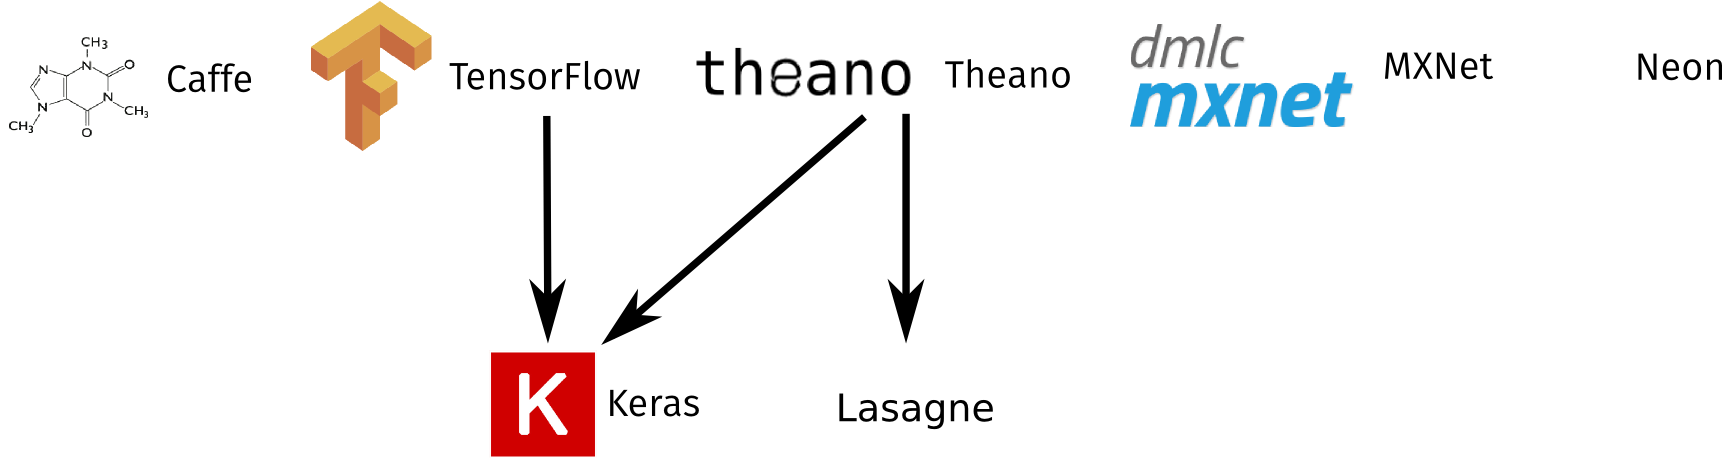
\includegraphics[width=\textwidth]{dl_frameworks_python}
\end{figure}
\begin{itemize}
	\item Beaucoup de frameworks
    \item Performances à peu près équivalentes
\end{itemize}
\end{frame}

\begin{frame}{\textit{Frameworks} Python}
\begin{block}{Les frameworks}
Utilisent C++ et CUDA en \textit{back-end}
\begin{itemize}
	\item Caffe (Berkeley), orienté "images"
    \item TensorFlow (Google)
    \item Theano (U. Montréal)
    \item Neon (Nervana Systems)
\end{itemize}
\end{block}

\begin{block}{Les surcouches}
\begin{itemize}
    \item Keras : surcouche pour Theano et TensorFlow
    \item Lasagne : surcouche pour Theano
\end{itemize}
\end{block}
\end{frame}

\begin{frame}{Matériel}

\begin{columns}

\begin{column}{0.80\textwidth}
\begin{block}{GPU recommandé}
Les réseaux de neurones sont \textbf{très} gourmands en calcul mais bien adaptés au traitement parallèle sur GPU (notamment pour les convolutions).
\begin{itemize}
	\item Avantage notable à NVIDIA
    \item Implémentations rapides avec CUDA/CuDNN
    \item $\approx$ 10x plus rapide sur GPU vs CPU
\end{itemize}
\end{block}
\end{column}

\begin{column}{0.20\textwidth}
\begin{figure}

\includegraphics[width=\textwidth]{python}\\
\Huge{$+$}\\
\vspace{1em}
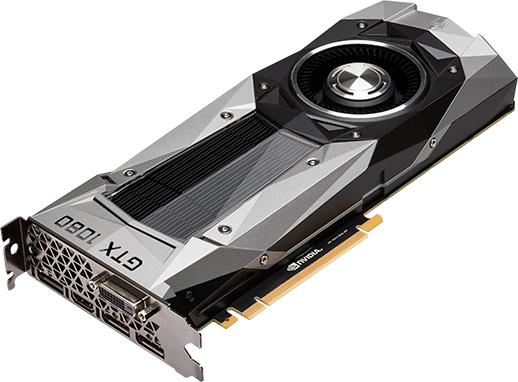
\includegraphics[width=\textwidth]{gpu}
\end{figure}
\end{column}

\end{columns}

\end{frame}

\begin{frame}{\textit{Setup}}

\begin{enumerate}
	\item Installer CUDA/CuDNN
    \item Installer Python
    \item \texttt{pip install keras} (Theano par défaut)
\end{enumerate}

\end{frame}

\begin{frame}[fragile]{À quoi ça ressemble ?}
Avec Keras :
\begin{figure}
	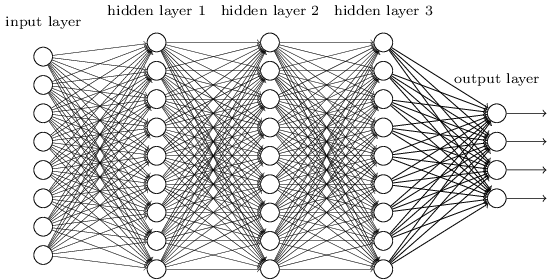
\includegraphics[width=\textwidth]{fully_connected}
\end{figure}
\end{frame}

\begin{frame}[fragile]{À quoi ça ressemble ?}
\begin{minted}[fontsize=\small]{python}
from keras.models import Sequential
from keras.layers import Dense
model = Sequential()
# input 32*32 flattened image
model.add(Dense(4096,input_dim=32*32,activation='relu'))
model.add(Dense(4096,activation='relu'))
model.add(Dense(4096,activation='relu'))
model.add(Dense(10,activation='softmax'))
# Compile model
model.compile(loss='categorical_crossentropy',
       optimizer='adam', metrics=['accuracy'])
# Fit the model
model.fit(X_train,y_train,nb_epoch=10,batch_size=200)
\end{minted}
\end{frame}

\begin{frame}[fragile]{À quoi ça ressemble ?}
Avec Keras :
\begin{figure}
	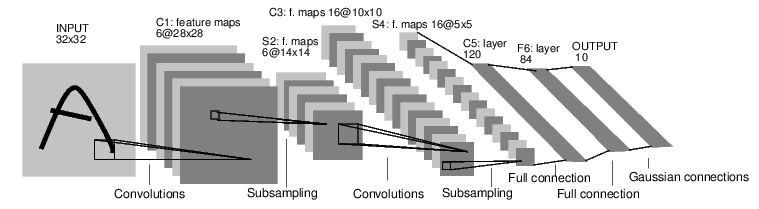
\includegraphics[width=\textwidth]{lenet5}
\end{figure}
\end{frame}

\begin{frame}[fragile]{À quoi ça ressemble ?}
\begin{minted}[fontsize=\small]{python}
from keras.models import Sequential
from keras.layers import Dense, Activation, Flatten
from keras.layers import Convolution2D, MaxPooling2D

model = Sequential()
# input: 32x32 images with 3 channels
model.add(Convolution2D(32, 3, 3, input_shape=(3, 32, 32)))
model.add(Activation('relu'))
model.add(MaxPooling2D(pool_size=(2, 2)))
model.add(Convolution2D(32, 3, 3))
model.add(Activation('relu'))
model.add(MaxPooling2D(pool_size=(2, 2)))
\end{minted}
\end{frame}

\begin{frame}[fragile]{À quoi ça ressemble ?}
\begin{minted}[fontsize=\small]{python}
# Flatten the feature maps
model.add(Flatten())
model.add(Dense(256))
model.add(Activation('relu'))
# 26 output classes (e.g. alphabet)
model.add(Dense(26))
model.add(Activation('softmax'))

model.compile(loss='categorical_crossentropy',
              optimizer='adam')

model.fit(X_train, Y_train, batch_size=32, nb_epoch=1)
\end{minted}
\end{frame}

\section{Pour aller plus loin}
\begin{frame}{Les concepts avancés}  
Modèles génératifs (créer des images, de la musique\dots aléatoirement !)

\begin{figure}
	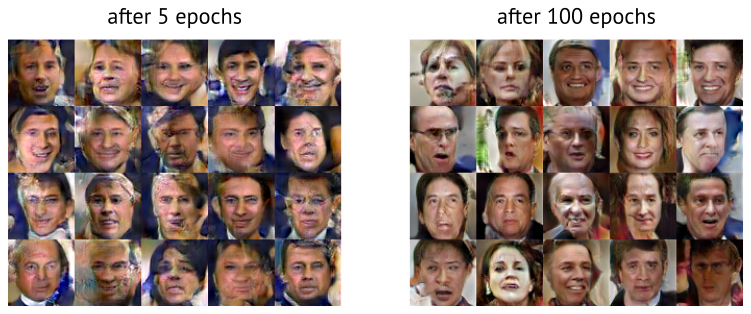
\includegraphics[width=\textwidth]{gan_faces}
\end{figure}
\end{frame}

\begin{frame}{Les concepts avancés}
Apprentissage par renforcement (AlphaGo, Space Invaders, Doom\dots)

\begin{figure}
	
\includegraphics[width=0.8\textwidth]{alphago}
\end{figure}

\end{frame}

\begin{frame}{Ressources pour débuter}
En français
\begin{itemize}
	\item Cours de Yann LeCun au \href{https://www.college-de-france.fr/site/yann-lecun/course-2015-2016.htm}{Collège de France}
    \item \href{https://fr.coursera.org/learn/neural-networks}{MOOC "Réseaux de neurones"} par G. Hinton (Coursera)
\end{itemize}
En anglais
\begin{itemize}
	\item \textit{Deep Learning} par Goodfellow et al.
    \item Documentation Caffe (notebooks)
    \item \small \url{https://github.com/ChristosChristofidis/awesome-deep-learning}
    \item \small \url{https://github.com/kjw0612/awesome-deep-vision}
\end{itemize}
\end{frame}

\begin{frame}{Fin}
\begin{block}{Questions ?}
Et réponses ?
\end{block}

\begin{exampleblock}{Contact}
\texttt{nicolas+python@audebert.at}
\end{exampleblock}
\end{frame}

\end{document}
